% Credits are indicated where needed. The general idea is based on a template by Vel (vel@LaTeXTemplates.com) and Frits Wenneker.

\documentclass[11pt, a4paper]{article} % General settings in the beginning (defines the document class of your paper)
% 11pt = is the font size
% A4 is the paper size
% “article” is your document class

%----------------------------------------------------------------------------------------
%	Packages
%----------------------------------------------------------------------------------------

% Necessary
\usepackage[german,english]{babel} % English and German language 
\usepackage{booktabs} % Horizontal rules in tables 
% For generating tables, use “LaTeX” online generator (https://www.tablesgenerator.com)
\usepackage{comment} % Necessary to comment several paragraphs at once
\usepackage[utf8]{inputenc} % Required for international characters
\usepackage[T1]{fontenc} % Required for output font encoding for international characters

% Might be helpful
\usepackage{amsmath,amsfonts,amsthm} % Math packages which might be useful for equations
\usepackage{tikz} % For tikz figures (to draw arrow diagrams, see a guide how to use them)
\usepackage{tikz-cd}
\usetikzlibrary{positioning,arrows} % Adding libraries for arrows
\usetikzlibrary{decorations.pathreplacing} % Adding libraries for decorations and paths
\usepackage{tikzsymbols} % For amazing symbols ;) https://mirror.hmc.edu/ctan/graphics/pgf/contrib/tikzsymbols/tikzsymbols.pdf 
\usepackage{blindtext} % To add some blind text in your paper


%---------------------------------------------------------------------------------
% Additional settings
%---------------------------------------------------------------------------------

%---------------------------------------------------------------------------------
% Define your margins
\usepackage{geometry} % Necessary package for defining margins

\geometry{
	top=2cm, % Defines top margin
	bottom=2cm, % Defines bottom margin
	left=2.2cm, % Defines left margin
	right=2.2cm, % Defines right margin
	includehead, % Includes space for a header
	%includefoot, % Includes space for a footer
	%showframe, % Uncomment if you want to show how it looks on the page 
}

\setlength{\parindent}{15pt} % Adjust to set you indent globally 

%---------------------------------------------------------------------------------
% Define your spacing
\usepackage{setspace} % Required for spacing
% Two options:
\linespread{1.5}
%\onehalfspacing % one-half-spacing linespread

%----------------------------------------------------------------------------------------
% Define your fonts
\usepackage[T1]{fontenc} % Output font encoding for international characters
\usepackage[utf8]{inputenc} % Required for inputting international characters

\usepackage{XCharter} % Use the XCharter font


%---------------------------------------------------------------------------------
% Define your headers and footers

\usepackage{fancyhdr} % Package is needed to define header and footer
\pagestyle{fancy} % Allows you to customize the headers and footers

%\renewcommand{\sectionmark}[1]{\markboth{#1}{}} % Removes the section number from the header when \leftmark is used

% Headers
\lhead{STAT 333} % Define left header
\chead{\textit{}} % Define center header - e.g. add your paper title
\rhead{Regression Runner} % Define right header

% Footers
\lfoot{} % Define left footer
\cfoot{\footnotesize \thepage} % Define center footer
\rfoot{ } % Define right footer

%---------------------------------------------------------------------------------
%	Add information on bibliography
\usepackage{natbib} % Use natbib for citing
\usepackage{har2nat} % Allows to use harvard package with natbib https://mirror.reismil.ch/CTAN/macros/latex/contrib/har2nat/har2nat.pdf

% For citing with natbib, you may want to use this reference sheet: 
% http://merkel.texture.rocks/Latex/natbib.php

%---------------------------------------------------------------------------------
% Add field for signature (Reference: https://tex.stackexchange.com/questions/35942/how-to-create-a-signature-date-page)
\newcommand{\signature}[2][5cm]{%
  \begin{tabular}{@{}p{#1}@{}}
    #2 \\[2\normalbaselineskip] \hrule \\[0pt]
    {\small \textit{Signature}} \\[2\normalbaselineskip] \hrule \\[0pt]
    {\small \textit{Place, Date}}
  \end{tabular}
}
%---------------------------------------------------------------------------------
%	General information
%---------------------------------------------------------------------------------
\title{title} % Adds your title
\author{
Stanley Zheng \space Eric \space Lucas
% Add your first and last name
    \thanks{Equal contribution} % Adds a footnote to your title
    %\institution{YOUR INSTITUTION} % Adds your institution
  }

\date{\small \today} % Adds the current date to your “cover” page; leave empty if you do not want to add a date


%---------------------------------------------------------------------------------
%	Define what’s in your document
%---------------------------------------------------------------------------------

\begin{document}


% If you want a cover page, uncomment "%---------------------------------------------------------------------------------
% Cover page
%---------------------------------------------------------------------------------

% Here are more templates for other cover pages: https://www.latextemplates.com/cat/title-pages

% This example is based on this cover page example: https://www.latextemplates.com/template/academic-title-page

\begin{titlepage} % Starts new environment where the page number is not displayed and the count starts at 1 for the next page

%------------------------------------------------
%	Institutional information
%------------------------------------------------
	
\begin{minipage}{0.4\textwidth} % Begins new environment (like a text box)
    \begin{flushleft} % Sets environment on the left side of the paper
    \large
    University of XX\\ % Add your institution
    Chair of Political Science IV\\ % Add the chair
    Fall 2018\\ % Add term
    COURSE TITLE\\ % Add course title
    Supervisor: NAME % Add instructor/supervisor name 
    \end{flushleft}
\end{minipage}
	
\vspace*{2in} % Adds some space in-between
	
\center % Centre everything on the page

%------------------------------------------------
%	Main part
%------------------------------------------------
	
{\huge\bfseries 值jij}\\[0.4cm] % Add your paper title 
{\large\today}\\[0.4cm] % Add date (current day)
FIRSTNAME LASTNAME % Add your name
	
\vfill % Adds additional space

%------------------------------------------------
%	General information about the author
%------------------------------------------------

\vfill % Adds additional space

Your contact info \\ % Add your contact info
Your Program \\ % Add info about your program
Semester you are enrolled \\ % Add info about your semester

\vfill % Adds additional space

%------------------------------------------------
%	Word count
%------------------------------------------------

\vfill % Adds additional space
	
Word count: XXXX % To indicate the word count
% How to check words in a LaTeX document: https://www.overleaf.com/help/85-is-there-a-way-to-run-a-word-count-that-doesnt-include-latex-commands
	

	
\end{titlepage}" and uncomment "\begin{comment}" and "\end{comment}" to comment the following lines
%%---------------------------------------------------------------------------------
% Cover page
%---------------------------------------------------------------------------------

% Here are more templates for other cover pages: https://www.latextemplates.com/cat/title-pages

% This example is based on this cover page example: https://www.latextemplates.com/template/academic-title-page

\begin{titlepage} % Starts new environment where the page number is not displayed and the count starts at 1 for the next page

%------------------------------------------------
%	Institutional information
%------------------------------------------------
	
\begin{minipage}{0.4\textwidth} % Begins new environment (like a text box)
    \begin{flushleft} % Sets environment on the left side of the paper
    \large
    University of XX\\ % Add your institution
    Chair of Political Science IV\\ % Add the chair
    Fall 2018\\ % Add term
    COURSE TITLE\\ % Add course title
    Supervisor: NAME % Add instructor/supervisor name 
    \end{flushleft}
\end{minipage}
	
\vspace*{2in} % Adds some space in-between
	
\center % Centre everything on the page

%------------------------------------------------
%	Main part
%------------------------------------------------
	
{\huge\bfseries 值jij}\\[0.4cm] % Add your paper title 
{\large\today}\\[0.4cm] % Add date (current day)
FIRSTNAME LASTNAME % Add your name
	
\vfill % Adds additional space

%------------------------------------------------
%	General information about the author
%------------------------------------------------

\vfill % Adds additional space

Your contact info \\ % Add your contact info
Your Program \\ % Add info about your program
Semester you are enrolled \\ % Add info about your semester

\vfill % Adds additional space

%------------------------------------------------
%	Word count
%------------------------------------------------

\vfill % Adds additional space
	
Word count: XXXX % To indicate the word count
% How to check words in a LaTeX document: https://www.overleaf.com/help/85-is-there-a-way-to-run-a-word-count-that-doesnt-include-latex-commands
	

	
\end{titlepage}

%\begin{comment}
\maketitle % Print your title, author name and date; comment if you want a cover page 

% \begin{center} % Center text
%     Word count: XXXX
% % How to check words in a LaTeX document: https://www.overleaf.com/help/85-is-there-a-way-to-run-a-word-count-that-doesnt-include-latex-commands
% \end{center}
%\end{comment}

%----------------------------------------------------------------------------------------
% Abstract
%----------------------------------------------------------------------------------------
\setcounter{page}{1} % Sets counter of page to 1
\section{Abstract} % Adds a section title
This project investigates how the relationship between three-point shooting and team success 
in the NBA has evolved over the past two decades. Using team-level data from the 2003-04 and 
2023-24 regular seasons obtained via the NBA API, we construct multiple linear regression 
models to examine the effects of three-point percentage (3P\%), two-point percentage (2P\%), 
and shot selection proportions on win rate. Our analysis reveals a statistically significant 
interaction between 3P\% and era, indicating that the marginal impact of three-point accuracy 
on team success has increased substantially in the modern NBA. While 3P\% showed no significant 
association with win rate in 2003-04, it has become a strong predictor in 2023-24—even after 
controlling for other efficiency metrics. This shift reflects a broader structural change in 
league strategy, marking the emergence of a “three-point era.” Though based on observational 
data, the use of interaction terms allows for a quasi-causal interpretation of this evolving 
relationship.
%----------------------------------------------------------------------------------------
% Introduction
%----------------------------------------------------------------------------------------
\section{Introduction} % Add a section title
\subsection{Motivation} % Add a subsection title
Over the past two decades, the NBA has undergone a dramatic transformation in offensive strategy. 
The rise of “small-ball” systems and analytics-driven decision making has led to a surge in 
three-point attempts, reshaping how teams space the floor, select shots, and build rosters. 
Players like Stephen Curry have redefined the value of long-range shooting, prompting coaches 
and front offices to reconsider the role of the three-point shot in winning games. This project 
is motivated by a key question at the heart of this shift: Has the importance of three-point 
shooting truly increased over time, and if so, how does it compare to traditional metrics like 
two-point efficiency or shot selection proportions? By using regression analysis on team-level 
data from different seansons, we aim to quantify how the statistical relationship 
between shooting performance and win rate has changed. In the era of big data, we believe that 
understanding these evolving dynamics can help teams identify actionable areas for improvement 
and optimize offensive strategies for greater success.
\subsection{Dataset}
Our dataset is sourced from the NBA's public API, an online interface that provides comprehensive 
and standardized statistics for teams and players across multiple seasons. The NBA API offers detailed 
data covering a wide range of performance categories, including shooting statistics, rebounding, passing, 
turnovers, fouls, player efficiency metrics, and advanced team analytics.

The full dataset records team-level aggregates for each regular season, capturing key indicators such as 
field goal percentages, three-point and two-point shooting volume and accuracy, free throw statistics, 
rebound counts, assist counts, turnover rates, steal and block numbers, and overall team performance metrics 
like win-loss records and plus-minus ratings. The structure of the dataset is shown in the Figure \ref{fig:original_data}, and the 
detailed explanation of each variable is shown in the Appendix.
\begin{figure}[htbp]
    \centering
    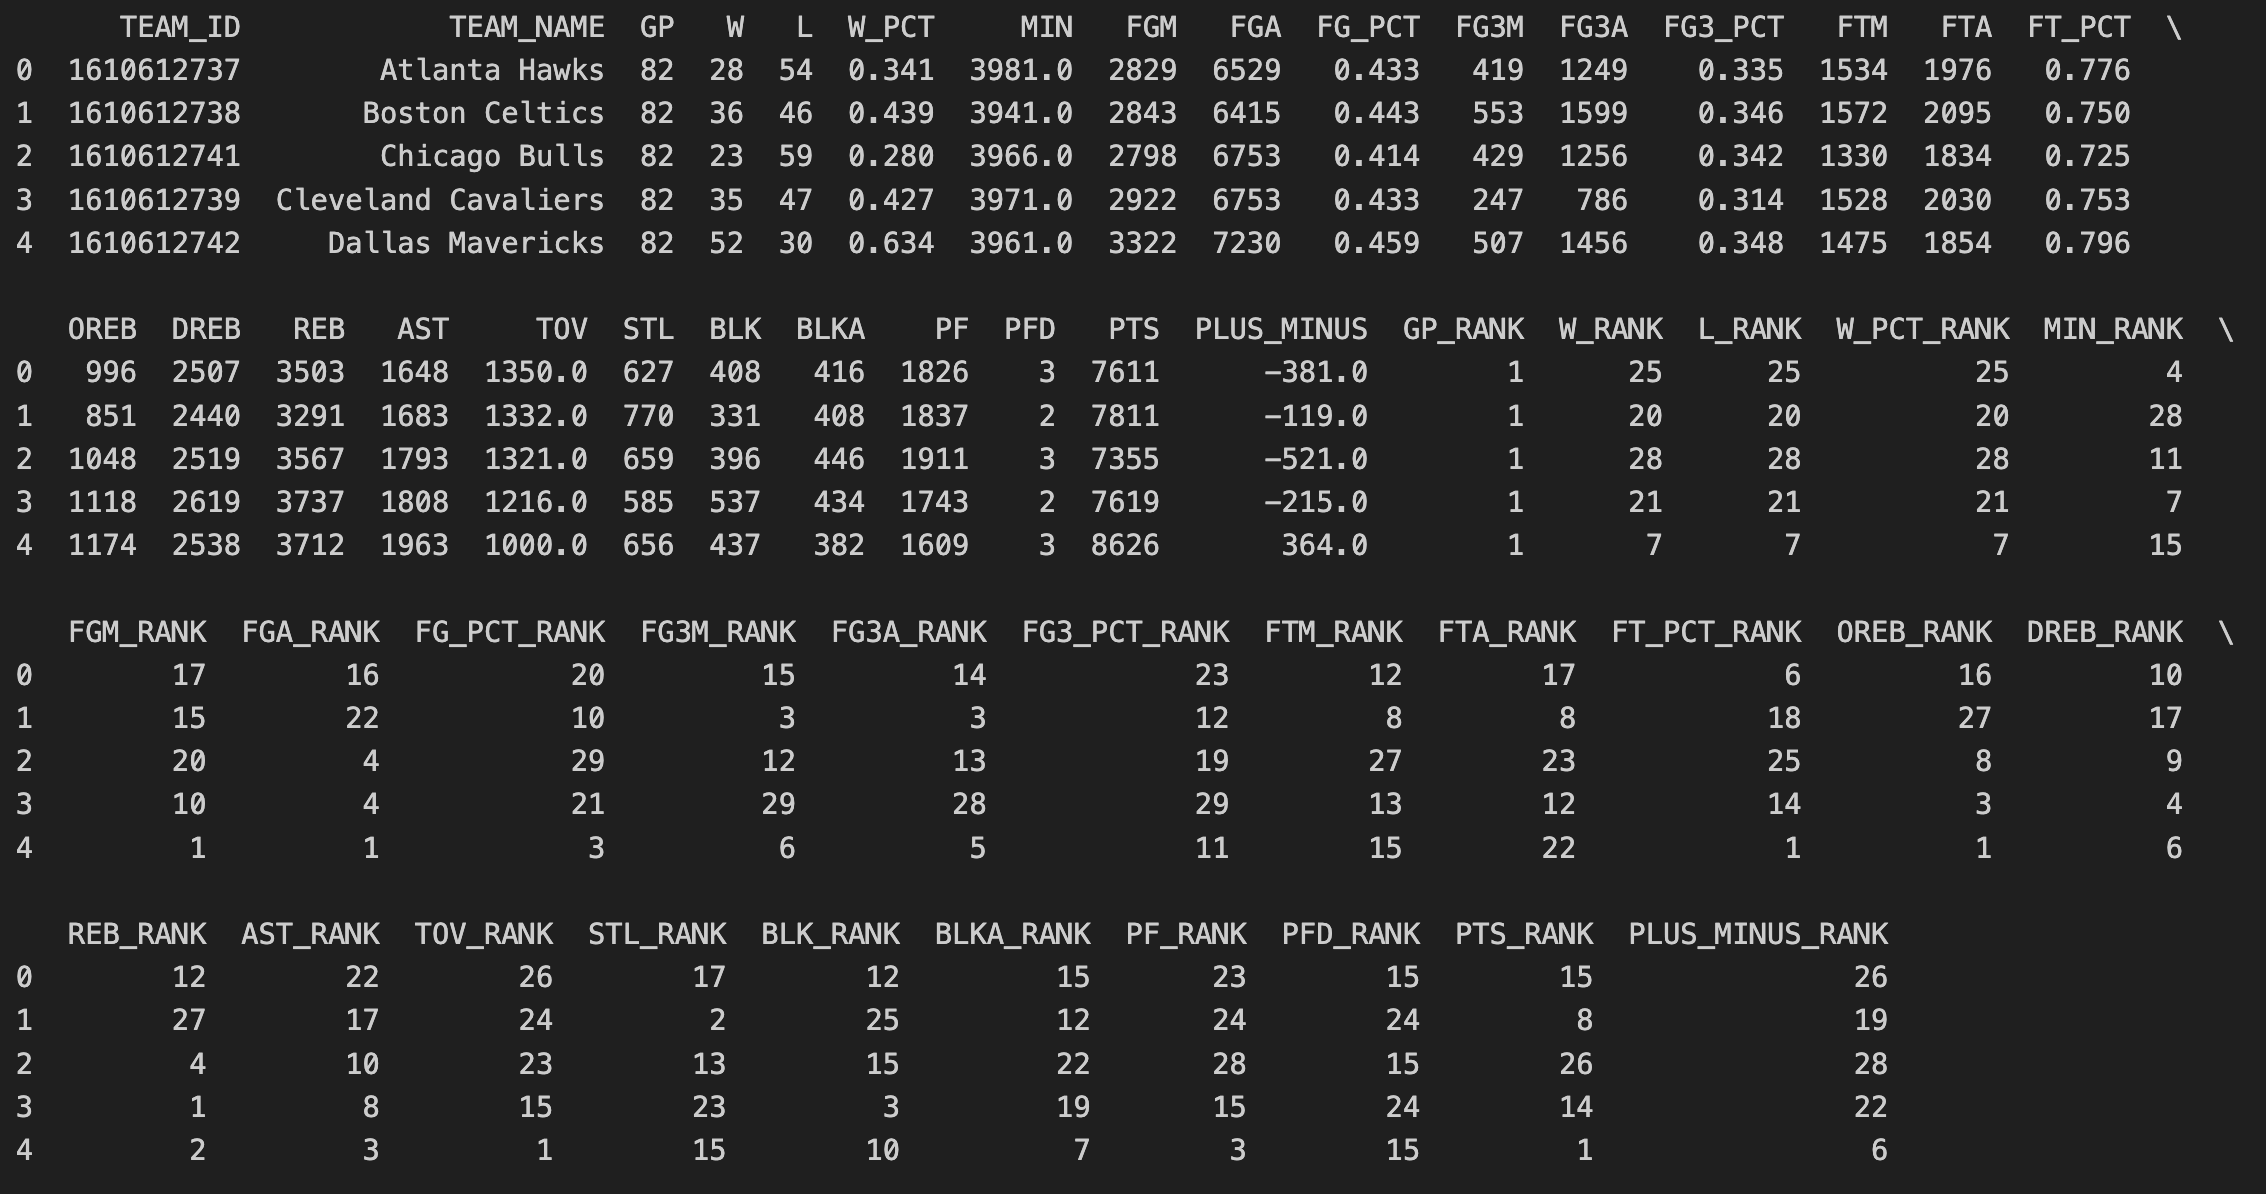
\includegraphics[width=0.9\textwidth]{figure/original_data.png}
    \caption{The Description of The Original Dataset.}
    \label{fig:original_data}
\end{figure}

For our analysis, we primarily focus on shooting-related metrics, including three-point field goal percentage (3P\%), 
two-point field goal percentage (2P\%), three-point attempt rate (3PA rate), and two-point attempt rate (2PA rate). 
Three-point and two-point attempt rates are computed as the proportion of total field goal attempts originating from 
each respective shot zone. To control for other aspects of team strength that may confound the relationship between 
shooting performance and win rate, we also incorporate variables such as total rebounds, turnovers, and other 
team-level performance indicators as covariates in our regression models. This approach allows us to better isolate 
the specific impact of shooting metrics on team success across different eras.
% Some example text
% \LaTeX allows you to highlight text in various ways: \textbf{bold}, \textit{italics}, with \textsc{small caps} or \texttt{as a coding font}.\footnote{ This command adds a footnote to your text.} 
% Citing in \LaTeX is easy. You could easier cite with the text flow like this ``Referring to \citet{collier2004greed} ...''  or at the end of the sentence \cite{collier2004greed}. You can also cite pages like this \citep[55]{collier2004greed}. If you want to add an additional note, you might want to do it this way \citep[cp.][22]{collier2004greed} or like this \citep[cp.][]{collier2004greed}.\\

%----------------------------------------------------------------------------------------
% Data Analysis
%----------------------------------------------------------------------------------------

\section{Data Analysis}
\subsection{Data Preprocess}

\subsection{Data Visulization}

%---------------------------------------------------------------------------------
% Model
%---------------------------------------------------------------------------------

\section{Model}

\subsection{Model Dianostic}

%----------------------------------------------------------------------------------------
% Conclusion
%----------------------------------------------------------------------------------------

\section{Conclusion}

\newpage % Includes a new page

\pagenumbering{roman} % Changes page numbering to roman page numbers
%\bibliography{literature}

\bibliography{literature.bib} % Add the filename of your bibliography
\bibliographystyle{apsr} % Defines your bibliography style

% For citing, please see this sheet: http://merkel.texture.rocks/Latex/natbib.php

% %----------------------------------------------------------------------------------------
% % Appendix
% %----------------------------------------------------------------------------------------
% \newpage % Includes a new page
% \section*{Appendix} % Stars disable section numbers
% % \appendix % Uncomment if you want to add an "automatic" appendix
% \pagenumbering{Roman} % Changes page numbering to Roman page numbers

% \blindtext % Adds some blind text

% %----------------------------------------------------------------------------------------
% % Declaration
% %----------------------------------------------------------------------------------------
% \newpage % Includes a page break
% \thispagestyle{empty} % Leaves the page style empty (no page number, no header, no footer)
% \section*{Statutory Declaration} % Stars disable section numbers

% \begin{otherlanguage}{german}
% Hiermit versichere ich, dass diese Arbeit von mir pers\"{o}nlich verfasst ist und dass ich keinerlei fremde Hilfe in Anspruch genommen habe. Ebenso versichere ich, dass diese Arbeit oder Teile daraus weder von mir selbst noch von anderen als Leistungsnachweise andernorts eingereicht wurden. W\"{o}rtliche oder sinngem\"{a}{\ss}e \"{U}bernahmen aus anderen Schriften und Ver\"{o}ffentlichungen in gedruckter oder elektronischer Form sind gekennzeichnet. S\"{a}mtliche Sekund\"{a}rliteratur und sonstige Quellen sind nachgewiesen und in der Bibliographie aufgef\"{u}hrt. Das Gleiche gilt f\"{u}r graphische Darstellungen und Bilder sowie f\"{u}r alle Internet-Quellen. Ich bin ferner damit einverstanden, dass meine Arbeit zum Zwecke eines Plagiatsabgleichs in elektronischer Form anonymisiert versendet und gespeichert werden kann. Mir ist bekannt, dass von der Korrektur der Arbeit abgesehen und die Pr\"{u}fungsleistung mit nicht ausreichend bewertet werden kann, wenn die Erkl\"{a}rung nicht erteilt wird.
% \end{otherlanguage}

% \vspace*{1in} % Adds extra space between two paragraphs

% \noindent I hereby declare that the paper presented is my own work and that I have not called upon the help of a third party. In addition, I affirm that neither I nor anybody else has submitted this paper or parts of it to obtain credits elsewhere before. I have clearly marked and acknowledged all quotations or references that have been taken from the works of others. All secondary literature and other sources are marked and listed in the bibliography. The same applies to all charts, diagrams and illustrations as well as to all Internet resources. Moreover, I consent to my paper being electronically stored and sent anonymously in order to be checked for plagiarism. I am aware that the paper cannot be evaluated and may be graded ``failed'' (``nicht ausreichend'') if the declaration is not made.\\

% %\vspace*{1in} % Adds extra space

% % Add field for signature, date, and place
% \hfill \signature{} 


% %---------------------------------------------------------------------------------

\end{document}
